\documentclass[12pt,a4paper]{article}
\usepackage{cmap} % Makes the PDF copiable. See http://tex.stackexchange.com/a/64198/25761
\usepackage[T1]{fontenc}
\usepackage[brazil]{babel}
\usepackage[utf8]{inputenc}
\usepackage{amsmath}
\usepackage{amsfonts}
\usepackage{amssymb}
\usepackage{amsthm}
\usepackage{textcomp} % \degree
\usepackage{gensymb} % \degree
\usepackage[usenames,svgnames,dvipsnames]{xcolor}
\usepackage{hyperref}
\usepackage{multicol}
\usepackage{graphicx}
\usepackage[margin=2cm]{geometry}
\usepackage{systeme}
\usepackage{icomma}

\hypersetup{
    colorlinks = true,
    allcolors = {blue}
}

% TODO: Consider using exsheets
% http://linorg.usp.br/CTAN/macros/latex/contrib/exsheets/exsheets_en.pdf
%
% http://ctan.org/tex-archive/macros/latex/contrib/exercise/
% Options: answerdelayed,lastexercise,noanswer
\usepackage[answerdelayed,lastexercise]{exercise}

\addto\captionsbrazil{%
\def\listexercisename{Lista de exerc\'icios}%
\def\ExerciseName{Exerc\'icio}%
\def\AnswerName{Solu\c{c}\~ao do exerc\'icio}%
\def\ExerciseListName{Ex.}%
\def\AnswerListName{Solu\c{c}\~ao}%
\def\ExePartName{Parte}%
\def\ArticleOf{de\ }%
}

\renewcommand{\ExerciseHeaderTitle}{(\ExerciseTitle)\ }
\renewcommand{\ExerciseListHeader}{%\ExerciseHeaderDifficulty%
\textbf{%\ExerciseListName\
\ExerciseHeaderNB.\ %
%\ --- \
\ExerciseHeaderTitle}%
%\ExerciseHeaderOrigin
\ignorespaces}
\renewcommand{\AnswerListHeader}{\textbf{\ExerciseHeaderNB.\ (\AnswerListName)\ }}
\newcommand*\diff{\mathop{}\!\mathrm{d}}

\renewcommand{\theenumi}{\alph{enumi}}
\renewcommand\labelenumi{(\theenumi) }

\newcommand*\tipo{Prova III}
\newcommand*\turma{CCI192-04U}
\newcommand*\disciplina{ANN0001}
\newcommand*\eu{Helder G. G. de Lima}
\newcommand*\data{05/07/2024}

\author{\eu}
\title{\tipo - \disciplina}
\date{\data}

\begin{document}
\thispagestyle{empty}
\newgeometry{margin=2cm,bottom=0.5cm}
\begin{center}

\includegraphics[width=9.0cm]{marca} \\
\textbf{\tipo\ (\disciplina / \turma)} \\
Prof. \eu\footnote{
Este é um material de acesso livre distribuído sob os termos da licença \href{https://creativecommons.org/licenses/by-sa/4.0/deed.pt_BR}{Creative Commons BY-SA 4.0}}
\end{center}

\noindent Nome do(a) aluno(a): \underline{\hspace{9,7cm}} Data: \underline{\data}

%\section*{Instruções}
\begin{center}\fbox{
\begin{minipage}{14cm}
\begin{footnotesize}
\begin{itemize}
\renewcommand{\theenumi}{\Roman{enumi}}
\item Identifique-se em todas as folhas.
\item Mantenha o celular e os demais equipamentos eletrônicos desligados durante a prova.
\item Justifique cada resposta com cálculos ou argumentos baseados na teoria estudada.
\item Resolva $5$ das $6$ questões (deixe claro que questão não deverá ser corrigida).
\end{itemize}
\end{footnotesize}
\end{minipage}
}
\end{center}

%\section*{Questões}
\begin{ExerciseList}
\Exercise[title={2,0}] Obtenha a função afim que melhor se ajusta (no sentido dos mínimos quadrados) aos pontos do conjunto
\[
D = {(-6, -2), (-3, -1), (4, 2), (5, 4)},
\]
e calcule o resíduo quadrático da função obtida.

{\color{blue} \textit{(Utilize números decimais com 2 dígitos após a vírgula)}}

\Answer Sejam $P_1 = (-6, -2)$, $P_2 = (-3, -1)$, $P_3 = (4, 2)$ e $P_4 = (5, 4)$ e denote $g_1(x) = 1$ e $g_2(x) = x$. Para encontrar uma função da forma $q(x) = a_1 g_1(x) + a_2 g_2(x)$ que melhor se ajusta aos pontos $P_i = (x_i,y_i)$, para $1 \leq i \leq 4$, basta resolver o sistema $A^T A X = A^T B$, em que
\[
A
= \begin{bmatrix}
g_1(x_1) & g_2(x_1) \\
g_1(x_2) & g_2(x_2) \\
g_1(x_3) & g_2(x_3) \\
g_1(x_4) & g_2(x_4) \\
\end{bmatrix}
= \begin{bmatrix}
1 & x_1 \\
1 & x_2 \\
1 & x_3 \\
1 & x_4 \\
\end{bmatrix},
\quad
X =
\begin{bmatrix}
a_1\\a_2
\end{bmatrix},
\quad
B = \begin{bmatrix}
y_1 \\
y_2 \\
y_3 \\
y_4 \\
\end{bmatrix},
\]
Considerando os dados fornecidos, tem-se:
\[
A^T A
= \begin{bmatrix}
 4                  & \sum_{i=1}^4 x_i   \\
\sum_{i=1}^4 x_i    & \sum_{i=1}^4 x_i^2
\end{bmatrix}
=\begin{bmatrix}
 1 & 1 & 1 & 1 \\
-6 & -3 & 4 & 5
\end{bmatrix}
\cdot
\begin{bmatrix}
  1 & -6\\
  1 & -3\\
  1 & 4\\
  1 & 5
\end{bmatrix}
=\begin{bmatrix}
4 & 0 \\
0 & 86
\end{bmatrix},
\]
e
\[
A^T B
= \begin{bmatrix}
 \sum_{i=1}^4 y_i     \\
 \sum_{i=1}^4 x_i y_i
\end{bmatrix}
= \begin{bmatrix}
 1 & 1 & 1 & 1 \\
-6 & -3 & 4 & 5
\end{bmatrix}
\begin{bmatrix}
-2 \\ -1 \\ 2 \\ 4
\end{bmatrix}
= \begin{bmatrix}
3 \\ 43
\end{bmatrix}.
\]
Então,
$
A^T A X = A^T B
\Leftrightarrow
\begin{bmatrix}
4 & 0 \\
0 & 86
\end{bmatrix}
\cdot
\begin{bmatrix}
a_1\\
a_2
\end{bmatrix}
=
\begin{bmatrix}
3 \\ 43
\end{bmatrix}
\Leftrightarrow
\begin{bmatrix}
a_1\\
a_2
\end{bmatrix}
=
\begin{bmatrix}
3/4\\
1/2
\end{bmatrix}.
$

Portanto, a função é $q(x) = \frac{1}{2}x + \frac{3}{4}$, isto é, $q(x) = 0,5x + 0,75$. O resíduo quadrático é dado por
\[
R = \sum_1^4 (q(x_i) - y_i)^2
  = (-2,25 + 2)^2 + (-0,75 + 1)^2 + (2,75 - 2)^2 + (3,25 - 4)^2 = 1,25.
\]
\Exercise[title={2,0}] Sabendo que
$I = \int_{0}^{4} \sqrt{t} \diff{t}
= \frac{16}{3}
\approx 5,333$,
verifique que o erro absoluto (em módulo) da aproximação de $I$ pela regra de Gauss-Legendre com três pontos é menor do que $0,03$.

{\color{blue} \textit{(Utilize números decimais com 3 dígitos após a vírgula)}}

\Answer

Fazendo a mudança de variáveis $t = \frac{4 - 0}{2}x + \frac{0 + 4}{2} = 2x + 2$, tem-se $\diff{t} = 2\diff{x}$ e
$\int_{0}^{4} \sqrt{t} \diff{t} = 2\int_{-1}^1 \sqrt{2x + 2}\diff{x}$. Além disso,

\begin{itemize}
  \item Se $x = -0,775$, então $\sqrt{t} = \sqrt{2\cdot(-0,775) + 2} \approx 0,671$
  \item Se $x =  0,000$, então $\sqrt{t} = \sqrt{2\cdot  0,000  + 2} \approx 1,414$
  \item Se $x = +0,775$, então $\sqrt{t} = \sqrt{2\cdot  0,775  + 2} \approx 1,884$
\end{itemize}

Então, aplicando o método de Gauss-Legendre, obtém-se:
\begin{align*}
I & \approx
  2 \cdot (0,556 \cdot 0,671 + 0,889 \cdot 1,414 + 0,556 \cdot 1,884) \\
& = 2 \cdot (0,373 + 1,257 + 1,048)
  = 2 \cdot 2,678
  = 5,356
\end{align*}

Assim, $\varepsilon_{abs} = |5,333 - 5,356| = 0,023 < 0,3$.


\Exercise[title={2,0}] Utilize a regra de Newton-Cotes aberta de três pontos para calcular $\int_{0}^{1} \frac{\ln(x)}{x-1} \diff{x}$.

{\color{blue} \textit{(Utilize números decimais com 4 dígitos após a vírgula)}}

\Answer Seja $f(x) = \frac{\ln(x)}{x-1}$, considere o passo $h = \frac{1 - 0}{2 + 2} = \frac{1}{4} = 0,25$, e denomine os extremos do intervalo como $x_{-1} = 0$ e $x_3 = 1$. Então:
\begin{itemize}
  \item $x_0 = 0 + 1 \cdot 0,25 = 0,25$, e portanto $f(x_0) = \frac{\ln(0,25)}{0,25-1} \approx 1,8484$
  \item $x_1 = 0 + 2 \cdot 0,25 = 0,5$, e portanto $f(x_1) = \frac{\ln(0,5)}{0,5-1} \approx 1,3863$
  \item $x_2 = 0 + 3 \cdot 0,25 = 0,75$, e portanto $f(x_2) = \frac{\ln(0,75)}{0,75-1} \approx 1,1507$
\end{itemize}

Assim, pela regra de Newton-Cotes aberta de três pontos, obtém-se:
\begin{align*}
  \int_{0}^{1} \frac{\ln(x)}{x-1} \diff{x}
  & \approx \frac{4 \cdot 0,25}{3} \cdot \left[ 2\cdot 1,8484 - 1,3863 + 2\cdot 1,1507 \right]
    \approx \frac{1}{3} \cdot 4,6119
    \approx 1,5373
\end{align*}

\Exercise[title={2,0}] Mostre que a solução aproximada do problema de valor inicial
\[
\begin{cases}
y^\prime(x) = 10\cdot x \cdot y(x) , \quad x \in [0,000, 0,600]\\
y(0,000) = 0,100
\end{cases}
\]
pelo método de Euler explícito, com passo $h=0,200$ produz erros absolutos cada vez maiores (em módulo) ao longo do intervalo $[0,000, 0,600]$. Considere que a solução exata é $y(x) = \frac{1}{10}e^{5x^2}$.

{\color{blue} \textit{(Utilize números decimais com 3 dígitos após a vírgula)}}

\Answer Denotando $f(x,y) = 10 x y$ e $h=0,200$, pode-se expressar a fórmula do método de Euler explícito da seguinte forma:
\[
y_{i+1}
= y_{i} + h f(x_{i}, y_{i})
= y_{i} + 0,2 \cdot \left( 10 x_{i} y_{i} \right)
= y_{i} + 2 x_{i} y_{i}
= (1 + 2x_{i}) y_{i}.
\]
Disto resulta que os valores obtidos a cada passo são os seguintes:

\medskip
\begin{center}
\begin{tabular}{ccrrr}
\hline
$i$ & $x_i$ & $y_i$ & $y_{exato}(x_i)$ & $\varepsilon_i = y_i-y_{exato}(x_i)$ \\ \hline
$0$ & $0,000$ & $0,100$ & $0,100$ & $ 0,000$ \\
$1$ & $0,200$ & $0,100$ & $0,122$ & $-0,022$ \\
$2$ & $0,400$ & $0,140$ & $0,223$ & $-0,083$ \\
$3$ & $0,600$ & $0,252$ & $0,605$ & $-0,353$ \\ \hline
\end{tabular}
\end{center}
\medskip
Em particular, percebe-se que o módulo dos erros absolutos cresce a cada passo:
\[
0 < 0,022 < 0,083 < 0,353.
\]

A figura a seguir mostra a solução exata e a solução aproximada pelo método de Euler:
\medskip
\begin{center}
\includegraphics[width=5.5cm]{img/prova-3-cci-euler-explícito.pdf}
\end{center}


\Exercise[title={2,0}] Seja $f(x) = \ln(x)$ no intervalo $[1, 5]$. Utilize as raízes do polinômio de Chebyshev de grau dois, e (se necessário) uma transformação do intervalo, para construir um polinômio interpolador de grau menor ou igual a um para $f(x)$.

{\color{blue} \textit{(Utilize números decimais com 3 dígitos após a vírgula)}}


\Answer O polinômio de Chebyshev de grau dois é dado por $T_2(x) = \cos(2\arccos(x)) = 2 x^2 - 1$ para $x \in [-1, 1]$, e suas raízes são
\[
x_1 = \cos\left(\frac{1}{4}\pi\right) = \frac{\sqrt{2}}{2} \approx 0,707
\text{ e }
x_2 = \cos\left(\frac{3}{4}\pi\right) = -\frac{\sqrt{2}}{2} \approx -0,707.
\]

Transformando o intervalo $[-1, 1]$ em $[1, 5]$ por meio da mudança de variáveis
\[
\tilde{x} = \frac{1}{2}[(5-1)x + (1+5)] = 2x + 3,
\]
obtém-se $\tilde{x}_1 \approx 4,414$ e $\tilde{x}_2 \approx 1,586$. Por Lagrange, o polinômio $p(x)$ que interpola $f(x) = \ln(x)$ nesses pontos é dado por:
\begin{align*}
p(x)
& = \ln(4,414) \left(\frac{x - 1,586}{4,414 - 1,586}\right)
+ \ln(1,586) \left(\frac{x - 4,414}{1,586 - 4,414}\right)\\
& = 0,525 (x - 1,586) - 0,163 (x - 4,414)
  = 0,362 x - 0,113.
\end{align*}

\Exercise[title={2,0}] Use o método de Runge-Kutta de 2ª ordem para resolver o problema de valor inicial
\[
\begin{cases}
y^\prime(x) = -y(x)/x \\
y(1) = y_0 = 28.
\end{cases}
\]
com passo $h=3$, no intervalo $[1, 7]$. Qual é o erro absoluto da aproximação em $x=7$, considerando que a solução exata é dada por $y = 28/x$?

{\color{blue} \textit{(Utilize números decimais com 2 dígitos após a vírgula)}}

\Answer
Com $f(x,y) = -y/x$,
$k_1 = f(x_i, y_i)$,
$k_2 = f(x_i + h, y_i + k_1 h)$, e
$y_{i+1} = y_i + \frac{h}{2} (k_1 + k_2)$, obtém-se:
\medskip
\begin{center}
    \begin{tabular}{crrrr}
    \hline
       $i$ & $x_i$  & $y_i$ & $k_1$ & $k_2$ \\
    \hline
    0 & 1 & 28 & -28,00 & 14,00 \\
    1 & 4 &  7 &  -1,75 & -0,25 \\
    2 & 7 &  4 &  - & - \\
    \hline
    \end{tabular}
\end{center}
\medskip
Assim, o erro é $\varepsilon = y_2 - y(x_2) = 4 - 28/7 = 0$. A figura a seguir mostra a solução exata e a aproximação pelo método de Runge-Kutta de ordem 2:
\medskip
\begin{center}
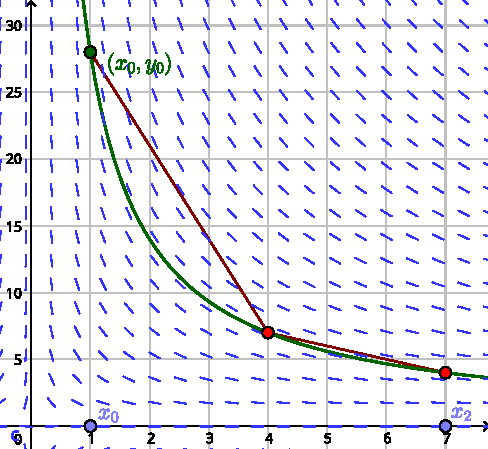
\includegraphics[width=5.5cm]{img/prova-3-cci-runge-kutta-2.pdf}
\end{center}
\end{ExerciseList}

\begin{center}
BOA PROVA E BOAS FÉRIAS!
\end{center}

\newpage
\restoregeometry
\section*{Respostas}
\shipoutAnswer
\end{document}
